
% frame 00
\begin{frame}
	\frametitle{Elementi di Codifica dei Caratteri}
	\framesubtitle{Definizioni}
	\addtocounter{nframe}{1}

	\begin{block}{Rappresentare il testo in formato digitale}
		L’adozione di metodologie informatiche per il trattamento dei testi richiede in primo luogo di fornire un'adeguata  rappresentazione dei dati testuali in formato digitale.
	\end{block}

\end{frame}

% frame 01
\begin{frame}
	\frametitle{Elementi di Codifica dei Caratteri}
	\framesubtitle{Definizioni}
	\addtocounter{nframe}{1}

	\begin{block}{Perché è importante}
		La codifica dei caratteri costituisce il grado zero della rappresentazione di testi su supporto digitale.
		\\ Essa costituisce la base di tutti gli ulteriori sistemi di codifica testuale.
	\end{block}



	\begin{block}{Codifica dei caratteri}
		%Capitolo sul character encoding e modulo Ganji 
		Come qualsiasi altro tipo di dato, anche i caratteri vengono rappresentati all’interno di un elaboratore mediante una codifica numerica binaria.
		\\Le codifiche dei caratteri sono la base di qualsiasi schema di codifica testuale.
	\end{block}

\end{frame}

% frame 02
\begin{frame}
	\frametitle{Elementi di Codifica dei Caratteri}
	\framesubtitle{Definizioni}
	\addtocounter{nframe}{1}

	% \begin{block}{Character set, Code Set}
	%  - Character set
	%  - Code Set
	%  - Character encoding
	%  - Tabella del Code page
	% \end{block}

	\begin{description}
		\item [Character set] spiega ...
		\item [Code Set] spiega ...
		\item [Character encoding] spiega ...
		\item [Tabella del Code page] spiega ...
		\item [Unicode] spiega
	\end{description}

\end{frame}

% frame 03
\begin{frame}
	\frametitle{Elementi di Codifica dei Caratteri}
	\framesubtitle{Definizioni}
	\addtocounter{nframe}{1}

	\begin{block}{Tabella Code Page ASCII 7 bit}
		%immagine di esempio Code Page ASCII (cp1252)
		\begin{center}
			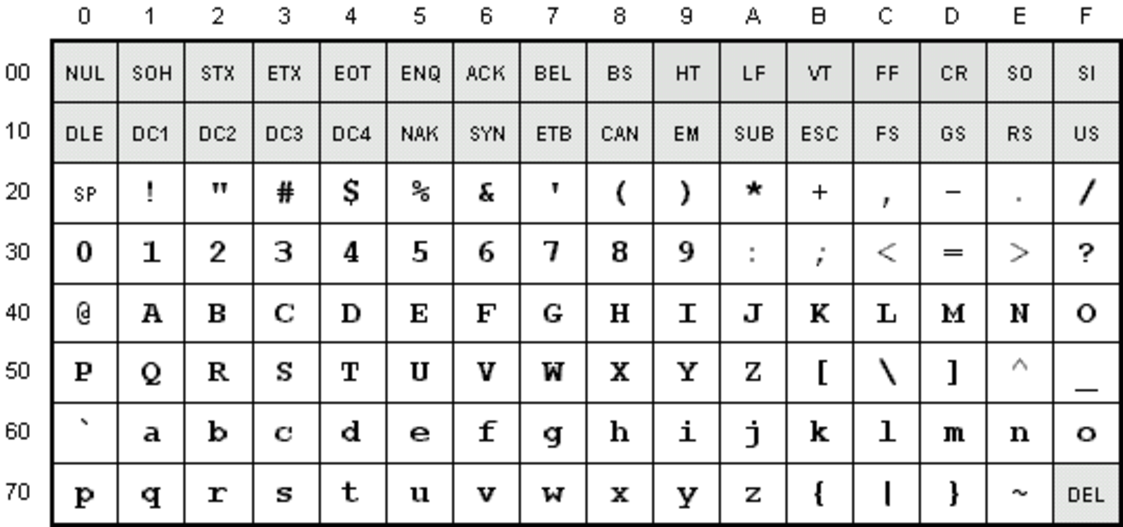
\includegraphics[width=.9\textwidth]{imgs/ascii-67.pdf}
		\end{center}

	\end{block}
	%\hline
	\begin{tiny}
		\begin{center}
			7 bit = 128 possibili caratteri; 32 caratteri di controllo; 96 caratteri effettivi
		\end{center}

	\end{tiny}

\end{frame}

% frame 0
\begin{frame}
	\frametitle{Elementi di Codifica dei Caratteri}
	\framesubtitle{Esempio codifica binaria}
	\addtocounter{nframe}{1}

	\begin{block}{codifica \textit{ciao mondo!} 7 bit ASCII}
		\begin{center}
			\textsc{6369 616f 206d 6f6e 646f 210a}
		\end{center}
	\end{block}

	\begin{block}{codifica \textit{ciao è mondo!} 8 bit ASCII}
		\begin{center}
			\textmd{6369 616f 20\textbf{e8} 206d 6f6e 646f 210a       }
		\end{center}
	\end{block}

	\begin{block}{codifica \textbf{ciao è mondo!} UNICODE UTF-8}
		\begin{center}
			6369 616f 20\textbf{c3 a8}20 6d6f 6e64 6f21 0a
		\end{center}
	\end{block}

\end{frame}


% frame 0
\begin{frame}
	\frametitle{Elementi di Codifica dei Caratteri}
	\framesubtitle{Complessità e rappresentazione}
	\addtocounter{nframe}{1}

	\begin{block}{Complessità di rappresentazione universale dei caratteri}
		Se si considerano tutti i possibili alfabeti del mondo e le molteplici esigenze poste dalla scrittura delle fonti manoscritte antiche e medievali, ci si accorge che la realizzazione di un sistema universale per la codifica dei caratteri è un progetto molto complesso con svariate sfide da affrontare.
	\end{block}

\end{frame}


\begin{frame}
	\frametitle{Elementi di Codifica dei Caratteri}
	\framesubtitle{Unicode}
	\addtocounter{nframe}{1}

	\begin{block}{Complessità di rappresentazione universale}
		Cenno al consorzio Unicode
	\end{block}

\end{frame}

